\documentclass[a4paper,12pt]{article}
\usepackage[top = 2.5cm, bottom = 2.5cm, left = 2.5cm, right = 2.5cm]{geometry}
\usepackage[T1]{fontenc}
\usepackage[utf8]{inputenc}
\usepackage{multirow} 
\usepackage{booktabs} 
\usepackage{graphicx}
\usepackage[spanish]{babel}
\usepackage{setspace}
\setlength{\parindent}{0in}
\usepackage{float}
\usepackage{fancyhdr}
\usepackage{amsmath}
\usepackage{amssymb}
\usepackage{amsthm}
\usepackage[numbers]{natbib}
\newcommand\Mycite[1]{%
	\citeauthor{#1}~[\citeyear{#1}]}
\usepackage{graphicx}
\usepackage{subcaption}
\usepackage{booktabs}
\usepackage{etoolbox}
\usepackage{minibox}
\usepackage{hyperref}
\usepackage{xcolor}
\usepackage[skins]{tcolorbox}
%---------------------------

\newtcolorbox{cajita}[1][]{
	 #1
}

\newenvironment{sol}
{\renewcommand\qedsymbol{$\square$}\begin{proof}[\textbf{Solución.}]}
	{\end{proof}}

\newenvironment{dem}
{\renewcommand\qedsymbol{$\blacksquare$}\begin{proof}[\textbf{Demostración.}]}
	{\end{proof}}

\newtheorem{problema}{Problema}
\newtheorem{definicion}{Definición}
\newtheorem{ejemplo}{Ejemplo}
\newtheorem{teorema}{Teorema}
\newtheorem{corolario}{Corolario}[teorema]
\newtheorem{lema}[teorema]{Lema}
\newtheorem{prop}{Proposición}
\newtheorem*{nota}{\textbf{NOTA}}
\renewcommand\qedsymbol{$\blacksquare$}
\usepackage{svg}
\usepackage{pgfplots}
\pgfplotsset{compat=1.11}

\usepackage{tikz}
\usetikzlibrary{calc}

\usetikzlibrary{patterns}
\usepackage[framemethod=default]{mdframed}
\global\mdfdefinestyle{exampledefault}{%
linecolor=lightgray,linewidth=1pt,%
leftmargin=1cm,rightmargin=1cm,
}




\newenvironment{noter}[1]{%
\mdfsetup{%
frametitle={\tikz\node[fill=white,rectangle,inner sep=0pt,outer sep=0pt]{#1};},
frametitleaboveskip=-0.5\ht\strutbox,
frametitlealignment=\raggedright
}%
\begin{mdframed}[style=exampledefault]
}{\end{mdframed}}
\newcommand{\linea}{\noindent\rule{\textwidth}{3pt}}
\newcommand{\linita}{\noindent\rule{\textwidth}{1pt}}

\AtBeginEnvironment{align}{\setcounter{equation}{0}}
\pagestyle{fancy}

\fancyhf{}









%----------------------------------------------------------
\lhead{\footnotesize Geometría diferencial}
\rhead{\footnotesize  Rudik Roberto Rompich}
\cfoot{\footnotesize \thepage}


%--------------------------

\begin{document}
 \thispagestyle{empty} 
    \begin{tabular}{p{15.5cm}}
    \begin{tabbing}
    \textbf{Universidad del Valle de Guatemala} \\
    Departamento de Matemática\\
    Licenciatura en Matemática Aplicada\\\\
   \textbf{Estudiante:} Rudik Roberto Rompich\\
   \textbf{Correo:}  \href{mailto:rom19857@uvg.edu.gt}{rom19857@uvg.edu.gt}\\
   \textbf{Carné:} 19857
    \end{tabbing}
    \begin{center}
        Geometría diferencial - Catedrático: Alan Reyes\\
        \today
    \end{center}\\
    \hline
    \\
    \end{tabular} 
    \vspace*{0.3cm} 
    \begin{center} 
    {\Large \bf  Tarea
} 
        \vspace{2mm}
    \end{center}
    \vspace{0.4cm}
%--------------------------
\begin{problema}
    Veamos un nuevo problema de calendarización. Tenemos un conjunto de tareas $S=\left\{a_{1}, \ldots, a_{n}\right\}$ donde la tarea $a_{i}$ tarda en realizarse $p_{i}$ de unidades de tiempo. Dependiendo de cómo calendaricemos su ejecución, cada tarea tendrá un tiempo de terminación $c_{i}$ (que es cuando la tarea se completa). Queremos hacer una calendarización non-preemptive (i.e., una tarea iniciada no se puede interrumpir) que minimice el promedio de todos los tiempos de terminación.
    \begin{enumerate}
        \item Proponga un algoritmo greedy que provea esta calendarización.
        \begin{sol}
            Se propone el siguiente algoritmo:
            \begin{verbatim}
function Greedy-Calendario(S, p)
    n = length(S)  # Obtiene el número de tareas

    # Ordena las tareas en orden ascendente de tiempo de ejecución
    for i = 1 to n
        for j = i+1 to n
            # Si el tiempo de ejecución de la tarea j 
            # es menor que el de la tarea i
            if p[j] < p[i]
                # Intercambia los tiempos de ejecución de las tareas i y j
                swap p[i] and p[j]
                # Intercambia las tareas i y j
                swap S[i] and S[j]

    # Inicializa el tiempo de terminación de las tareas
    c = [0]*n

    # Calcula el tiempo de terminación de cada tarea
    for i = 1 to n
        # El tiempo de terminación de la tarea i es la suma
        # del tiempo de terminación de la tarea anterior
        # y el tiempo de ejecución de la tarea i
        c[i] = c[i-1] + p[i]

    # Devuelve la secuencia de tareas y sus tiempos de terminación
    return S, c
            
            \end{verbatim}
        \end{sol}
        \item Determine el tiempo de ejecución de su algoritmo.
        \begin{sol}
            El algoritmo tiene dos bucles anidados que recorren todas las tareas, por lo que su tiempo de ejecución es $O(n^2)$, donde $n$ es el número de tareas.
        \end{sol}
        \item Demuestre que su algoritmo da la solución óptima (es decir, demuestre que el problema presenta las características que permiten obtener una solución óptima mediante un algoritmo greedy o, alternativamente, modele el problema como una matroide ponderada).
        \begin{sol}
    Podemos modelar este problema como una matroide ponderada. Las tareas son los elementos de la matroide, y el peso de cada tarea es su tiempo de ejecución. La función de peso es submodular, ya que el tiempo de ejecución total de cualquier subconjunto de tareas no puede ser mayor que el tiempo de ejecución total de todas las tareas. Tenemos: 

$$
\forall A, B \subseteq S, \quad A \subseteq B \implies w(A) \leq w(B)
$$

Donde $w(A)$ es la suma de los tiempos de ejecución de las tareas en $A$. Por lo tanto, el algoritmo greedy que selecciona la tarea con el menor tiempo de ejecución en cada paso es equivalente a un algoritmo que selecciona la tarea con el menor peso en cada paso en la matroide ponderada, lo que demuestra la optimalidad del algoritmo.
        \end{sol}
    \end{enumerate}



\end{problema}

\begin{problema}
    Demuestre que el minimum-spanning-tree problem y el problema de sitios de hospedaje descritos en clase se pueden modelar como matroides ponderadas (es decir, identifique y describa el conjunto $S$, la función de pesos y la familia de conjuntos independientes). Demuestre que cumplen con las propiedades de herencia e intercambio.
    \begin{dem}
        Una matroide ponderada es una pareja $M = (S, I)$ donde $S$ es un conjunto no vacío y $I$ es una familia de subconjuntos de $S$, llamados subconjuntos independientes. Además, existe una función de peso $w: S \rightarrow \mathbb{R}^+$ que asigna un valor positivo a cada elemento de $S$. La matroide debe cumplir con las siguientes propiedades:
        \begin{enumerate}
            \item Herencia: Si $A \in I$ y $B \subseteq A$, entonces $B \in I$.
            \item Propiedad de intercambio: Si $A, B \in I$ y $|B| > |A|$, entonces existe un $x \in B - A$ tal que $A \cup \{x\} \in I$.
        \end{enumerate}


        Ahora, demostraremos que el problema del árbol de expansión mínima (MST) y el problema de los sitios de hospedaje se pueden modelar como matroides ponderadas.

        \begin{itemize}
            \item (1) Minimum-spanning-tree problem:
            \begin{cajita}
                Este problema se da en el contexto de un grafo no dirigido, ponderado y conexo, denotado como $G(V,E)$, donde $V$ es el conjunto de vértices y $E$ es el conjunto de aristas. El objetivo es encontrar un árbol de expansión (un subgrafo que es un árbol, conecta todos los vértices y no tiene ciclos) con el peso mínimo posible. El peso de un árbol de expansión se calcula sumando los pesos de todas sus aristas. 
            \end{cajita}
            \begin{enumerate}
                \item Conjunto $S$: Este es el conjunto de todas las aristas en el grafo.
                \item Función de peso $w$: Esta es la función que asigna a cada arista un peso positivo.
                \item Familia de conjuntos independientes $I$: Esta es la colección de todos los subconjuntos de aristas que no forman un ciclo en el grafo.
                
            \end{enumerate}

            Propiedades:
            \begin{itemize}
                \item Herencia: Si $A \in I$ y $B \subseteq A$, entonces $B$ no puede contener un ciclo, porque $A$ no contiene un ciclo. Por lo tanto, $B \in I$.
                \item Propiedad de intercambio: Si $A, B \in I$ y $|B| > |A|$, entonces existe una arista $x \in B - A$ que puede ser añadida a $A$ sin formar un ciclo (porque $B$ es acíclico). Por lo tanto, $A \cup \{x\} \in I$.
            \end{itemize}
            \item (2) Problema de los sitios de hospedaje:
            \begin{cajita}
                Este problema se plantea como una página web para encontrar hospedaje, donde los lugares tienen una calificación calculada a partir de retroalimentación de antiguos clientes. La página desea proveer una funcionalidad que permita al usuario determinar un número $k$ y obtener los $k$ lugares de hospedaje cuya suma de calificaciones sea la más alta. En otras palabras, este problema desea el conjunto de $k$ lugares con calificaciones más altas (pues esto resultará en la suma más alta) de entre todos los disponibles.



            \end{cajita}
            \begin{enumerate}
                \item Conjunto $S$: Este es el conjunto de todos los lugares de hospedaje.
                \item Función de peso $w$: Esta es la función que asigna a cada lugar de hospedaje una calificación positiva.
                \item Familia de conjuntos independientes $I$: Esta es la colección de todos los subconjuntos de lugares de hospedaje de tamaño $k$ o menos.
                
            \end{enumerate}
            
            Propiedades:
            \begin{itemize}
                \item Herencia: Si $A \in I$ y $B \subseteq A$, entonces $|B| \leq |A| \leq k$. Por lo tanto, $B \in I$.
                \item Propiedad de intercambio: Si $A, B \in I$ y $|B| > |A|$, entonces existe un lugar de hospedaje $x \in B - A$ que puede ser añadido a $A$ sin exceder el tamaño $k$. Por lo tanto, $A \cup \{x\} \in I$.
            \end{itemize}
            
        \end{itemize}

        Por lo tanto, ambos problemas se pueden modelar como matroides ponderadas y cumplen con las propiedades de herencia e intercambio.


    \end{dem}

\end{problema}


\begin{problema}
    En una matroide $M=(S, I)$, donde $S$ tiene $n$ elementos, ¿qué puede asegurar sobre el tiempo de ejecución del algoritmo greedy correspondiente?
    \begin{sol}
        Consideremos la forma de los algoritmo Greedy: 
        \begin{figure}[H]
            \centering
            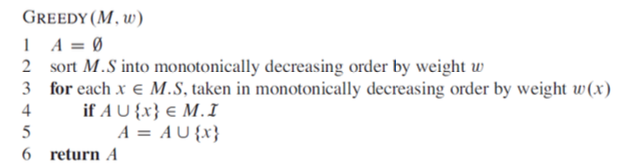
\includegraphics[scale=0.5]{Problemas/11.png}
        \end{figure}
        El tiempo de ejecución del algoritmo greedy en una matroide $M=(S, I)$, donde $S$ tiene $n$ elementos, depende de los valores de dos factores principales:
        \begin{enumerate}
            \item El tiempo necesario para ordenar el conjunto $S$ según la función de peso.
            \item El tiempo necesario para verificar si un conjunto es independiente.
        \end{enumerate}

    \end{sol}
\end{problema}


\begin{problema}
    Usted es catedrático de un curso libre en la UVG, y en su curso hay estudiantes de muchas carreras diferentes (cada estudiante, suponemos, perteneciente a una única carrera). La decanatura le ha solicitado seleccionar un equipo de estudiantes para enviar a una olimpiada de ciencias, con el requerimiento de no enviar a más de un estudiante de cada carrera. Los estudiantes participarán como equipo, y usted ha determinado que el equipo tendrá mejores posibilidades de ganar conforme más alta sea la suma de promedios de todos los miembros.
    \begin{enumerate}
        \item Demuestre que este problema se puede modelar como una matroide ponderada y provea el algoritmo greedy que lo resuelve.
        \begin{sol}
            Este problema se puede modelar como una matroide ponderada de la siguiente manera:
            \begin{itemize}
                \item Conjunto $S$: Este es el conjunto de todos los estudiantes en el curso.
                \item Función de peso $w$: Esta es la función que asigna a cada estudiante su promedio académico.
                \item Familia de conjuntos independientes $I$: Esta es la colección de todos los subconjuntos de estudiantes en los que no hay dos estudiantes de la misma carrera.
                
            \end{itemize}


Propiedades:
\begin{itemize}
    \item Herencia: Si $A \in I$ y $B \subseteq A$, entonces $B$ no puede tener dos estudiantes de la misma carrera, porque $A$ no tiene dos estudiantes de la misma carrera. Por lo tanto, $B \in I$.
    \item Propiedad de intercambio: Si $A, B \in I$ y $|B| > |A|$, entonces existe un estudiante $x \in B - A$ que puede ser añadido a $A$ sin que haya dos estudiantes de la misma carrera en $A \cup \{x\}$. Por lo tanto, $A \cup \{x\} \in I$.
\end{itemize}


Entonces, basado en la definición estándar de algoritmos greedy para resolver este problema sería el siguiente:
\begin{enumerate}
    \item Ordenar el conjunto $S$ en orden decreciente de promedio académico.
    \item Inicializar un conjunto vacío $A$.
    \item Recorrer cada estudiante $s$ en $S$ en orden. Si agregar $s$ a $A$ no resulta en dos estudiantes de la misma carrera en $A$, agregar $s$ a $A$.
    \item Devolver $A$
\end{enumerate}

        \end{sol}
        \item Desarrolle una instancia de este problema y úsela para ilustrar la aplicación de su algoritmo.
        \begin{sol}
             Supongamos que tenemos los siguientes estudiantes en el curso:
            \begin{itemize}
                \item Estudiante 1: Carrera A, promedio 85
                \item Estudiante 2: Carrera B, promedio 90
                \item Estudiante 3: Carrera C, promedio 80
                \item Estudiante 4: Carrera A, promedio 95
                \item Estudiante 5: Carrera B, promedio 88
            \end{itemize}


        Aplicamos el algoritmo:
        \begin{enumerate}
            \item Ordenamos los estudiantes: Estudiante 4, Estudiante 2, Estudiante 5, Estudiante 1, Estudiante 3.
            \item Inicializamos $A$ como un conjunto vacío.
            \item Recorremos cada estudiante en orden:
                \begin{enumerate}
                    \item Agregamos al Estudiante 4 a $A$.
                    \item Agregamos al Estudiante 2 a $A$.
                    \item No agregamos al Estudiante 5 a $A$ porque ya hay un estudiante de la Carrera B en $A$.
                    \item No agregamos al Estudiante 1 a $A$ porque ya hay un estudiante de la Carrera A en $A$.
                    \item Agregamos al Estudiante 3 a $A$.
                \end{enumerate}
               
            \item Devolvemos $A$, que contiene al Estudiante 4, Estudiante 2 y Estudiante 3.
        \end{enumerate}
        Con esto, podemos calcular la suma de los promedios de los estudiantes en el equipo, la cual es es 95 + 90 + 80 = 265. El conjunto $A$ que devuelve el algoritmo contiene a los estudiantes 4, 2 y 3. Este conjunto es el equipo de estudiantes que se enviará a la olimpiada de ciencias. Cada estudiante en este equipo es de una carrera diferente, cumpliendo con el requisito de la decanatura. Además, la suma de los promedios de estos estudiantes es la más alta posible, dado el requisito de que no puede haber más de un estudiante de la misma carrera.




        \end{sol}
    \end{enumerate}



\end{problema}


\begin{problema}
    El algoritmo de Dijkstra resuelve el problema del camino más corto entre dos vértices sobre un grafo ponderado positivamente y dirigido. Lo hace con un acercamiento greedy, mientras que el algoritmo de Bellman-Ford, discutido en los ejercicios del tema anterior, resuelve el mismo problema aplicando programación dinámica. Provea y compare (dicho de otra forma, investigue y discuta), con notación asintótica, cotas superiores a las tasas de crecimiento de los algoritmos de Dijkstra y Bellman-Ford. Suponiendo que ambos algoritmos se enfrentan a la misma instancia del problema, ¿cuál es mejor? Si no necesariamente se enfrentan a la misma instancia, ¿cuál es mejor?

    \begin{sol}
        Primero, definamos las complejidades de tiempo de los algoritmos de Dijkstra y Bellman-Ford. Usando la siguiente notación: $V$ son los nodos y $E$ las aristas.\bigbreak

El algoritmo de Dijkstra tiene una complejidad de tiempo de $O((V+E) \log V)$ cuando se implementa con una cola de prioridad binaria. Esto se debe a que cada vértice se extrae de la cola de prioridad una vez y cada arista se relaja una vez. Extraer un vértice de la cola de prioridad toma $O(\log V)$ y relajar una arista toma $O(1)$.\bigbreak

El algoritmo de Bellman-Ford tiene una complejidad de tiempo de $O(VE)$, ya que realiza $V-1$ iteraciones y en cada iteración, relaja todas las $E$ aristas.


\begin{center}
    \begin{tabular}{|c|c|}
        \hline
        Algoritmo & Complejidad de tiempo \\
        \hline
        Dijkstra & $O((V+E) \log V)$ \\
        Bellman-Ford & $O(VE)$ \\
        \hline
        \end{tabular}
\end{center}



En términos de complejidad de tiempo, el algoritmo de Dijkstra es generalmente más rápido que el algoritmo de Bellman-Ford, especialmente para grafos dispersos donde $E$ es mucho menor que $V^2$. Sin embargo, el algoritmo de Dijkstra solo funciona en grafos con pesos de aristas no negativos, mientras que el algoritmo de Bellman-Ford puede manejar grafos con pesos de aristas negativos.\bigbreak

Por lo tanto, si ambos algoritmos se enfrentan a la misma instancia del problema y se garantiza que todos los pesos de las aristas son no negativos, el algoritmo de Dijkstra sería la mejor opción. Si no se garantiza que todos los pesos de las aristas sean no negativos, entonces el algoritmo de Bellman-Ford sería la mejor opción, ya que puede manejar pesos de aristas negativos y detectar ciclos de peso negativo.
    \end{sol}
\end{problema}



%---------------------------
%\bibliographystyle{apa}
%\bibliography{referencias.bib}

\end{document}